\documentclass[a4paper,10pt]{article}

\usepackage{tikz}
\usepackage{fullpage}
\usepackage{amsmath,amsthm,amsfonts,amssymb,amscd}
\usepackage{mathtools}
\usepackage{colortbl}
\usepackage{xcolor}
\usepackage{graphicx}
\usepackage{titlesec}
\usepackage{xepersian}
\usepackage{multirow}
\usepackage{enumitem}


% ---------------------------
%      Dark Theme Setup
% ---------------------------
\definecolor{CustomBackground}{HTML}{1C1C1C}  % Dark background
\pagecolor{CustomBackground}
\color{white}

% ---------------------------
%        Font Setup
% ---------------------------
\settextfont{Vazir.ttf}[
BoldFont = Vazir-Bold.ttf,
Path = fonts/
]
\setlatintextfont{Vazir.ttf}[
BoldFont = Vazir-Bold.ttf,
Path = fonts/
]

% ---------------------------
%     Custom Adjustments
% ---------------------------
\renewcommand{\baselinestretch}{1.2}
\renewcommand{\thesection}{\arabic{section}}

% User-defined commands for homework info (adjust as needed)
\newcommand{\HomeworkNumber}{4}
\newcommand{\HomeworkDeadline}{1404/8/10}
\newcommand{\id}{\texttt{\detokenize{reza051taji}}}

\setlength{\parindent}{0pt}


\begin{document}
	
	% ---------------------------------
	%           Front Page
	% ---------------------------------
	\begin{titlepage}
		\begin{center}
			\vspace*{1cm}
			% Bigger Logo
			
\includegraphics[scale=1.1]{assets/fum-logo.png}\\[1cm]
			
			{\Huge \bfseries هوش مصنوعی پیشرفته}\\[0.5cm]
			{\Large دانشگاه فردوسی مشهد}\\[0.3cm]
			{\Large گروه مهندسی کامپیوتر}\\[0.5cm]
			{\normalsize دکتر هراتی}\\[2cm]
			
			 {\Huge \bfseries تمرین \HomeworkNumber}\\[0.5cm]
			{\Large مهلت تحویل: \HomeworkDeadline}\\[2.5cm]
			
			\Large مسئول تمرین: \id
			
		\end{center}
	\end{titlepage}
	
	% ---------------------------------
	%          Instructions
	% ---------------------------------
	\clearpage
	\section*{دستورالعمل‌ها}
	
	دانشجویان محترم لطفا به موارد زیر توجه فرمایید:
	\begin{itemize}
		\itemsep0em
		\item
		تحويل تمرين‌ها فقط از طريق سامانه  آموزش مجازی دانشگاه امکان‌‌پذیر است.
		\item 
		تمرین‌ها باید دست نویس، خوانا و با استفاده از خودکار آبی یا مشکی و یا به صورت دیجیتالی با استفاده از قلم نوری نوشته شوند. 
		\item
		از تمرین‌های حل شده دیگران و یا هوش مصنوعی استفاده نکنید. پیامد‌های این کار با دانشجو می‌باشد. 
		\item
		نوشتن جواب آخر به تنهايى نمره‌ای نداشته و تمام مراحل حل، مشمول نمره می‌باشد.
		\item 
		به دلیل موعد از پیش تعیین شده تمرین‌ها و برنامه درسی، امکان تمدید تمرین وجود ندارد. همچنین بدیهی است که ارسال تمرین پس از موعد تعیین شده نمره‌ای نخواهد داشت.
		
		\item نحوه نام‌گذاری فایل پاسخ باید مطابق جدول 1
		و به شکل pdf باشد.
		
		\begin{table}[h]
			\centering
			\begin{tabular}{|c|c|}
				\hline
				\textbf{Format} & \texttt{StudentID-FullName-\#HwNo.pdf} \\
				\hline
				\textbf{Example} & \texttt{9876543210-Alan\_Turing-\#01.pdf} \\
				\hline
			\end{tabular}
			\caption{شیوه نام‌گذاری فایل‌ها}
			\label{tab:file_format}
		\end{table}
		
		
	\end{itemize}
	\rule{\linewidth}{0.4pt}
	
	
	%  هر سوال که گذاشته میشه، حما 3 خط آخر رو هم بعد از اتمام نوشتن سوال بگذارید.
	% \bigskip
	% \bigskip
	% \hline
	
	\section{سوال اول}
	
	درستی یا نادرستی گزاره‌های زیر را با ذکر دلیل مشخص کنید.
	
	\begin{enumerate}[label=\alph*)]
		\item اگر مقدار Utility برای گره ترمینال منجر به شکست منفی نباشد، الگوریتم Minimax درست عمل نمی‌کند.
		
		\item اگر بخواهیم تابع Evaluation تخمین خوبی از گره غیرترمینال بزند، کافی است مقدار آن کوچک‌تر از مقدار Utility برای گره شکست نباشد.
	\end{enumerate}
	
	\bigskip
	\hline
	
	
	\bigskip
	
	\section{سوال دوم}
	
	در نوعی مدل‌سازی از مسائل بازی‌ها با دو عامل، می‌توانیم عامل متخاصم را به‌جای یک عامل مستقل، جزوی از ویژگی‌های محیط در نظر بگیریم تا مسئله تک‌عاملی شود و سعی کنیم مسئله را با انجام جستجوهای هیوریستیک کلاسیک حل کنیم:
	
	\begin{enumerate}[label=\alph*)]
		\item این کار چه ویژگی‌ای را به ویژگی‌های محیط اضافه می‌کند؟ (با فرض اینکه این ویژگی قبلاً وجود نداشته است.)
		
		\item این روش چه ایرادانی ممکن است نسبت به روش استاندارد (Minimax) داشته باشد؟ (دو مورد را به همراه دلایل ذکر کنید.)
		
		\item درصورتی که بتوانیم تصمیمات عامل متخاصم را در هر وضعیتی با قطعیت پیش‌بینی کنیم، الگوریتمی در محیط تک‌عاملی ارائه کنید که مسیر بهینه را پیدا کند. (ذکر نام یک الگوریتم کافی نیست!)
	\end{enumerate}
	
	
	\bigskip
	\bigskip
	\hline
	
	
	\bigskip
	\section{سوال سوم}
	
	در الگوریتم Minimax همواره فرض بر این است که عامل متخاصم (Min) بهینه عمل می‌کند. اگر بدانیم در واقعیت این عامل تصمیم بهینه نمی‌گیرد، آیا این الگوریتم همواره بهترین حرکت را برای عامل Max انتخاب می‌کند؟ دلیل خود را توضیح دهید.
	
	\bigskip
	\bigskip
	\hline
	
	
	\bigskip
	
	\section{سوال چهارم}
	
	در محیطی ۳ عامل A \lr{،} B و C با هم بازی می‌کنند. عامل‌های A و B ممکن است در لحظه‌ای با هم مشارکت کنند و علیه عامل C باشند، اما در لحظات بعدی هیچ مشارکتی شکل نگیرد. در این شرایط بگویید:
	
	\begin{enumerate}[label=\alph*)]
		\item Minimax Value چگونه نوشته می‌شود؟
		
		\item سیاست انتخاب هر عامل در درخت Minimax چگونه است؟
	\end{enumerate}
	
	
	\bigskip
	\bigskip
	\hline
	
	
	\bigskip
	\section{سوال پنجم}
	
	در جستجوی هیوریستیک مقدار Evaluation هر گره تنها تابعی از همان گره بود، اما در Minimax این مقدار با توجه به گره‌های بعدی و از پایین به بالا محاسبه می‌شود:
	
	\begin{enumerate}[label=\alph*)]
		\item علت این تفاوت چیست؟
		
		\item مقدار Cutoff برابر چه مقداری باشد تا Minimax از این حیث شبیه جستجوی هیوریستیک شود؟ این کار چه مزایا و معایبی دارد؟
	\end{enumerate}
	
	\bigskip
	\bigskip
	\hline
	
	
	
	\bigskip
	\section{سوال ششم}
	
	مشکل مقدار Cutoff ثابت چیست؟ چگونه می‌توان به روش Cutoff \lr{،} روش Iterative Deepening را اضافه کرد و در مجموع با احتساب زمان و دقت عملکرد بهتری داشت؟
	
	\bigskip
	\bigskip
	\hline
	
	
	\bigskip
	\section{سوال هفتم}
	
	یک روش محاسبه Evaluation ترکیب خطی تعدادی از ویژگی‌ها در یک وضعیت است که در آن به هر ویژگی وزنی داده می‌شود و اعداد حاصل با هم جمع می‌شوند:
	
	\begin{enumerate}[label=\alph*)]
		\item معایب این روش چیست؟
		
		\item مسئله‌ای را ذکر کنید و روشی غیرخطی پیشنهاد بدهید و توضیح دهید که چرا نسبت به روش ترکیب خطی بهتر عمل می‌کند.
	\end{enumerate}
	

	\bigskip
	\bigskip
 	\hline
	
	
	\bigskip
	\section{سوال هشتم}
	
	درباره الگوریتم هرس آلفا-بتا به سوالات پاسخ دهید:
	
	\begin{enumerate}[label=\alph*)]
		\item شرط هرس شدن فرزندان برای گره‌های Min و Max را بنویسید.
		
		\item با اجرای الگوریتم برای درخت زیر، (۱) شاخه‌های هرس‌شده را همراه علت هرس شدنشان مشخص کنید و (۲) برای هر گره مقادیر آلفا یا بتا را از ابتدای اجرای الگوریتم تا خاتمه آن به ترتیب بنویسید.
	\end{enumerate}
	
	\begin{center}
		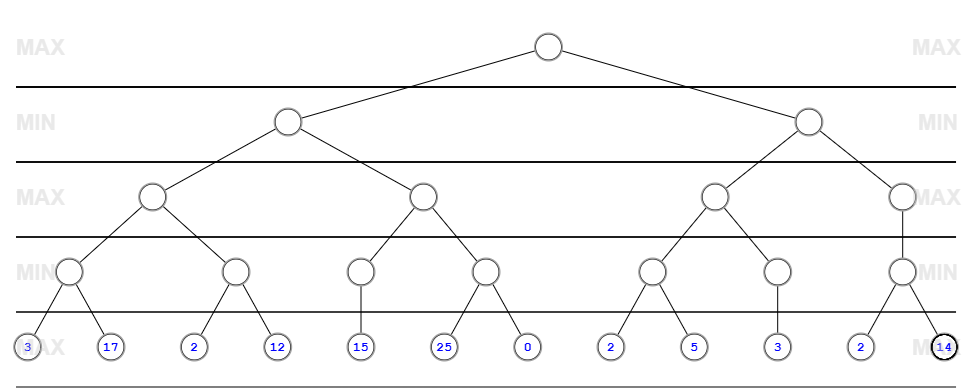
\includegraphics[width=0.8\textwidth]{assets/game-q8.png}
	\end{center}
	
	
	
	\bigskip
	\bigskip
	\hline
	
		\bigskip
	\section{سوال نهم}
	
	در بازی‌هایی که محیط غیرقطعی (Non-Deterministic) می‌باشد و شانس در آنها دخیل است (Stochastic-Games) از حالت تعمیم یافته الگوریتم Minimax به نام Expectiminimax استفاده می‌شود که علاوه بر گره‌های Min و Max، گره Chance نیز وجود دارد:
	
	\begin{enumerate}[label=\alph*)]
		\item در یک محیط قطعی مقدار یال‌های گره Chance چگونه باید باشد تا درخت Minimax تشکیل شود؟
		
		\item پیچیدگی زمانی Minimax و Expectiminimax در حالت ساده بدون Cutoff و هرس چگونه است؟ توضیح دهید.
		
		\item مقادیر هر گره زیر را با توجه به الگوریتم Expectiminimax به‌دست بیاورید.
	\end{enumerate}
	
	\begin{center}
		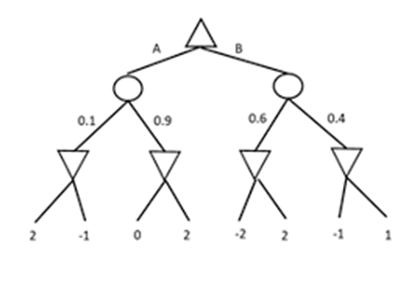
\includegraphics[width=0.6\textwidth]{assets/game-q9.png}
	\end{center}
	
	
	\bigskip
	\bigskip
	\hline
	
\end{document}



